\documentclass[dvipdfmx]{classes/tyukan}
\usepackage[final]{graphicx}

\Year{令和6}

\No{06}
\Name{糸川 倫太朗}
\Laboratory{青山研究室}

\Theme{A JavaScript compiler and TypeScript checker with a focus on
static analysis and runtime performance}
\Keywords{JavaScript, TypeScript, compiler, static analysis}

\begin{document}

\paragraph{<背景>}
AltJS として寡占的な立ち位置を獲得した TypeScript という言語がある.
その根幹となる TypeScript を JavaScript に変換するコンパイラ(\texttt{tsc})は,静的解析機や
language server に使用されてきた.
しかし,そんな \texttt{tsc} にはある問題がある.
それは, \texttt{tsc} による TypeScript の解析と型推論は非常に計算コストと時間コストが高いことである.
これにはいくつかの解決策があるが,どれも \texttt{tsc} に依存してしまうため,JavaScript
ランタイムの起動から実行までのボトルネックを無視できない.
そこで,本研究では \texttt{tsc} の代替となるパフォーマンスを意識したコンパイラを作成することにした.

\paragraph{<目的>}
language server や静的解析機で使用した際,\texttt{tsc} と比較して,高速でハイパフォーマンスなコンパイラを作成する.

\paragraph{<研究の概要>}
「decaf」と名付けた本研究は Rust を使用して開発する.
TypeScript のパースは \texttt{oxc\_parser} を参考に実装する.
型推論は \texttt{tsc} を参考に実装する.

\texttt{decaf} では \texttt{tsc} と異なった型推論のアーキテクチャを提案する.

\begin{figure}[h]
  \centering
  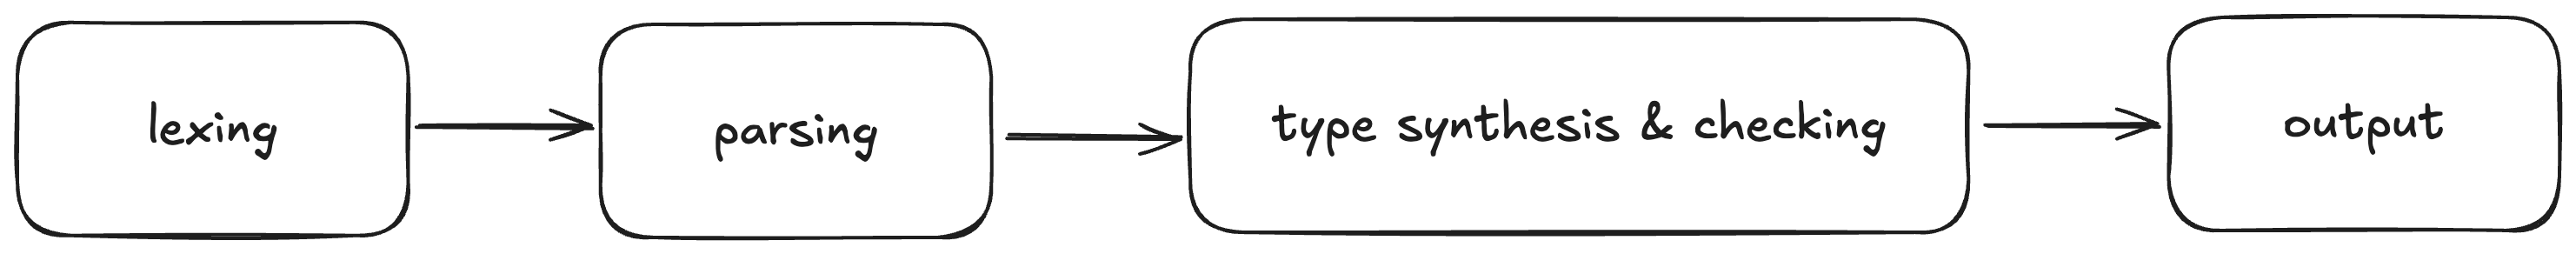
\includegraphics[width=0.9\columnwidth]{figures/type_check_arch.png}
  \caption{\texttt{tsc} の型推論アーキテクチャ}
  \label{fig:type_check_arch}
\end{figure}

図 \ref{fig:type_check_arch} は従来の TypeScript の型推論アーキテクチャである.
\texttt{decaf} では,このアーキテクチャのうち型の合成と検査の部分が \texttt{tsc} と異なる.

まず, \texttt{tsc} では型の合成と検査を同時に行うが, \texttt{decaf} では型の合成と検査を分離する.
型の合成を分離したのは,TypeScript の AST を \texttt{decaf} の型合成機が解釈できる形(TypeID
と呼ばれる)に変換する中間レイヤであり,本来型の合成機とは独立しているためである.

\texttt{decaf} では型合成機は,値と構造に関する情報を型として保持し,関数やブロックの振る舞いをイベントとしてエンコードする.
これにより,プログラム実行時のヒープのような役割を型検査時に果たすことができる.

\texttt{decaf} では型検査機は,\texttt{tsc} と異なったアプローチを取る.
\texttt{decaf} の型検査機では型を「その値が取りうる可能性の空間」として捉える.
これにより,実行時に起こりうるすべての可能性を型チェック時に考慮できる.

\paragraph{<研究の現状>}
現在, \texttt{decaf} は TypeScript のほぼ全ての構文をパースできる.

一方で型推論,検査は概要で述べたアーキテクチャに基づいて実装中である.

\paragraph{<今後の方針>}
サポートする構文を増やし,型推論の精度を向上させる.
また,プレイグラウンドを作成し,フィードバックを受けやすい環境を整える.

\end{document}
